% Prueba local: mismo preambulo del informe 2, solo con los archivos de circuitos.
% (logo, bibliografia y sub_files de los companeros no estan en este equipo)
    \documentclass[twocolumn]{IEEEtran}
    \usepackage[margin=1cm]{geometry}
    \usepackage[spanish,mexico]{babel}
    \selectlanguage{spanish}
    \usepackage[caption=false,font=footnotesize]{subfig}
    \usepackage{multirow}
    \usepackage{graphicx}
    \usepackage{booktabs}
    \usepackage{amsmath}
    \usepackage[utf8]{inputenc}
    \usepackage[T1]{fontenc}
    \usepackage{amsmath}
    \usepackage{enumerate}
    \usepackage{amsfonts}
    \usepackage{graphicx}
    \usepackage[american]{circuitikz}
    \usepackage{fancyhdr}
    \pagestyle{fancy}
    \setlength{\headheight}{14pt}
    \setlength{\headsep}{8pt}
    \usepackage{listings}
    \usepackage{xcolor}
    \usepackage{tikz}
    \renewcommand{\familydefault}{\sfdefault}
    \usepackage{amsfonts}
    \usepackage[hidelinks]{hyperref}
    \usepackage{float}
    \usepackage{titlesec}
    \setcounter{secnumdepth}{3}
    \setcounter{tocdepth}{3}
    \titleformat{\section}{\large\bfseries\filcenter}{\thesection}{1em}{}
    \titleformat{\subsection}{\normalsize\bfseries\filcenter}{\thesubsection}{0.75em}{}
    \titleformat{\subsubsection}{\normalsize\bfseries}{\thesubsubsection}{0.5em}{}
    \titleformat{\paragraph}[runin]{\bfseries\itshape}{}{0pt}{}[:]
    \usepackage{enumitem}
    \setlength{\parskip}{0.2em}
    \fancyhf{}
    \lhead{\footnotesize \textbf{ Informe $\#2$:} Caracterización de rectificadores de potencia con diodos  }
    \rhead{\footnotesize \today}
    \setlength{\textfloatsep}{10pt}
    \setlength{\floatsep}{8pt}
    \setlength{\intextsep}{8pt}
\begin{document}
\section{Procedimiento (prueba)}
% =====================================================================
%  Macros de los circuitos (CircuiTikZ ya se carga en el main con [american]).
%  Se puede \input en cualquier parte del documento antes de los circuitos.
% =====================================================================
\ctikzset{voltage dir=RP}

% ---- Etiquetas editables (cambiar con \renewcommand dentro de cada figura) ----
\providecommand{\etqFuente}{v_s}            % senal de entrada
\providecommand{\etqSec}{v_p}               % cada mitad del secundario (tab central)
\providecommand{\etqCarga}{R_L}             % resistencia de carga (reostato)
\providecommand{\etqSalida}{V_{out}}        % voltaje de salida
\providecommand{\etqCuno}{C_1}
\providecommand{\etqCdos}{C_2}
\providecommand{\etqRdummy}{1\,\Omega}      % valor de la R dummy
\providecommand{\sepCarga}{3.2}             % distancia R_L -> selector de C (subir si las etiquetas son largas)

% ---- Bloque: switch en paralelo con R dummy ----------------------------
% \dummyH{punto inicial}{largo}{switch}{resistencia}  horizontal, hacia la derecha
% \dummyV{punto inicial}{largo}{switch}{resistencia}  vertical, hacia abajo
\providecommand{\dummyH}[4]{%
  \draw (#1) to[short,*-] ++(0,0.6) to[nos, l={$#3$}] ++(#2,0) -- ++(0,-1.2)
             to[R, l={$#4$}] ++(-#2,0) -- ++(0,0.6);
  \draw (#1) ++(#2,0) node[circ]{};
}
\providecommand{\dummyV}[4]{%
  \draw (#1) to[short,*-] ++(-0.6,0) to[nos, l_={$#3$}] ++(0,-#2) -- ++(1.2,0)
             to[R, l_={$#4$}] ++(0,#2) -- ++(-0.6,0);
  \draw (#1) ++(0,-#2) node[circ]{};
}

% ---- Bloque: carga R_L con selector de capacitor en paralelo -----------
% \carga{nodo superior}{altura}{switch}
%   brazo al centro = abierto, izquierda = C1, derecha = C2
%   deja definida la coordenada (B) = nodo inferior de R_L
%   (flechas escritas como stealth-stealth para no chocar con babel-spanish)
\providecommand{\carga}[3]{%
  \coordinate (T) at (#1);
  \draw (T) to[vR, l_={$\etqCarga$}, v^={$\etqSalida$}, *-*] ++(0,-#2) coordinate(B);
  \draw (T) -- ++(\sepCarga,0) node[circ]{} coordinate(P) node[above]{$#3$};
  \draw[line width=0.8pt] (P) -- ++(0,-0.75);                          % brazo (abierto)
  \draw[stealth-stealth, thin] (P) ++(-125:0.55) arc[start angle=-125, end angle=-55, radius=0.55];
  \draw (P) ++(-0.7,-0.9) coordinate(K1) to[C, l_={$\etqCuno$}, o-*] (K1 |- B);
  \draw (P) ++( 0.7,-0.9) coordinate(K2) to[C, l={$\etqCdos$}, o-] (K2 |- B);
  \draw (B) -- (K2 |- B);
}

% ---- Transformador con tab central -------------------------------------
\providecommand{\trafoTab}{%
  \draw (0,0) to[sV, l={$\etqFuente$}] (0,4) -- (1.5,4) to[cute inductor] (1.5,0) -- (0,0);
  \draw[line width=1pt] (1.95,0.6) -- (1.95,3.4) (2.15,0.6) -- (2.15,3.4);
  \draw (2.6,4) to[cute inductor, mirror, l={$\etqSec$}] (2.6,2)
                to[cute inductor, mirror, l={$\etqSec$}] (2.6,0);
}

% =====================================================================
%  Circuitos generalizados (reemplazan las imagenes de los circuitos)
%  Requiere antes: % =====================================================================
%  Macros de los circuitos (CircuiTikZ ya se carga en el main con [american]).
%  Se puede \input en cualquier parte del documento antes de los circuitos.
% =====================================================================
\ctikzset{voltage dir=RP}

% ---- Etiquetas editables (cambiar con \renewcommand dentro de cada figura) ----
\providecommand{\etqFuente}{v_s}            % senal de entrada
\providecommand{\etqSec}{v_p}               % cada mitad del secundario (tab central)
\providecommand{\etqCarga}{R_L}             % resistencia de carga (reostato)
\providecommand{\etqSalida}{V_{out}}        % voltaje de salida
\providecommand{\etqCuno}{C_1}
\providecommand{\etqCdos}{C_2}
\providecommand{\etqRdummy}{1\,\Omega}      % valor de la R dummy
\providecommand{\sepCarga}{3.2}             % distancia R_L -> selector de C (subir si las etiquetas son largas)

% ---- Bloque: switch en paralelo con R dummy ----------------------------
% \dummyH{punto inicial}{largo}{switch}{resistencia}  horizontal, hacia la derecha
% \dummyV{punto inicial}{largo}{switch}{resistencia}  vertical, hacia abajo
\providecommand{\dummyH}[4]{%
  \draw (#1) to[short,*-] ++(0,0.6) to[nos, l={$#3$}] ++(#2,0) -- ++(0,-1.2)
             to[R, l={$#4$}] ++(-#2,0) -- ++(0,0.6);
  \draw (#1) ++(#2,0) node[circ]{};
}
\providecommand{\dummyV}[4]{%
  \draw (#1) to[short,*-] ++(-0.6,0) to[nos, l_={$#3$}] ++(0,-#2) -- ++(1.2,0)
             to[R, l_={$#4$}] ++(0,#2) -- ++(-0.6,0);
  \draw (#1) ++(0,-#2) node[circ]{};
}

% ---- Bloque: carga R_L con selector de capacitor en paralelo -----------
% \carga{nodo superior}{altura}{switch}
%   brazo al centro = abierto, izquierda = C1, derecha = C2
%   deja definida la coordenada (B) = nodo inferior de R_L
%   (flechas escritas como stealth-stealth para no chocar con babel-spanish)
\providecommand{\carga}[3]{%
  \coordinate (T) at (#1);
  \draw (T) to[vR, l_={$\etqCarga$}, v^={$\etqSalida$}, *-*] ++(0,-#2) coordinate(B);
  \draw (T) -- ++(\sepCarga,0) node[circ]{} coordinate(P) node[above]{$#3$};
  \draw[line width=0.8pt] (P) -- ++(0,-0.75);                          % brazo (abierto)
  \draw[stealth-stealth, thin] (P) ++(-125:0.55) arc[start angle=-125, end angle=-55, radius=0.55];
  \draw (P) ++(-0.7,-0.9) coordinate(K1) to[C, l_={$\etqCuno$}, o-*] (K1 |- B);
  \draw (P) ++( 0.7,-0.9) coordinate(K2) to[C, l={$\etqCdos$}, o-] (K2 |- B);
  \draw (B) -- (K2 |- B);
}

% ---- Transformador con tab central -------------------------------------
\providecommand{\trafoTab}{%
  \draw (0,0) to[sV, l={$\etqFuente$}] (0,4) -- (1.5,4) to[cute inductor] (1.5,0) -- (0,0);
  \draw[line width=1pt] (1.95,0.6) -- (1.95,3.4) (2.15,0.6) -- (2.15,3.4);
  \draw (2.6,4) to[cute inductor, mirror, l={$\etqSec$}] (2.6,2)
                to[cute inductor, mirror, l={$\etqSec$}] (2.6,0);
}

% =====================================================================
\begin{figure}[!t]
  \centering
  \resizebox{0.55\columnwidth}{!}{% 1) Rectificador de media onda
\begin{circuitikz}
  \draw (0,0) to[sV, l={$\etqFuente$}] (0,3)
        to[D*, l=$D_1$] (3.5,3)
        to[R, l_={$\etqCarga$}, v^={$\etqSalida$}] (3.5,0) -- (0,0);
  \draw (1.75,0) node[ground]{};
\end{circuitikz}
}
  \caption{Rectificador de media onda.}
  \label{fig:gen_media}
\end{figure}

\begin{figure}[!t]
  \centering
  \resizebox{\columnwidth}{!}{% 2) Rectificador de onda completa con tab central (2 diodos)
\begin{circuitikz}
  \trafoTab
  \draw (2.6,4) to[D*, l=$D_1$] (5,4) -- (6,4) -- (6,0);
  \draw (2.6,0) to[D*, l_=$D_2$] (5,0) -- (6,0);
  \draw (2.6,2) to[short,*-] (3.4,2) node[ground]{};
  \draw (6,2) to[short,*-] (7.6,2)
        to[R, l_={$\etqCarga$}, v^={$\etqSalida$}] (7.6,-0.5) node[ground]{};
\end{circuitikz}
}
  \caption{Rectificador de onda completa con tab central.}
  \label{fig:gen_tab}
\end{figure}

\begin{figure}[!t]
  \centering
  \resizebox{0.75\columnwidth}{!}{% 3) Puente rectificador (4 diodos)
\begin{circuitikz}
  \draw (0,0) to[D*, l=$D_2$] (0,2.2) to[D*, l=$D_1$] (0,4.4);
  \draw (3,0) to[D*, l=$D_4$] (3,2.2) to[D*, l=$D_3$] (3,4.4);
  \draw (0,2.2) to[sV, l={$\etqFuente$}, *-*] (3,2.2);
  \draw (0,4.4) to[short,-*] (3,4.4) -- (5,4.4)
        to[R, l_={$\etqCarga$}, v^={$\etqSalida$}] (5,0) to[short,-*] (3,0) -- (0,0);
  \draw (4,0) node[ground]{};
\end{circuitikz}
}
  \caption{Puente rectificador de onda completa.}
  \label{fig:gen_puente}
\end{figure}

% =====================================================================
%  Metodologia: montaje, bloques modulares, circuitos adaptados y mediciones
%  Uso en el main:  % =====================================================================
%  Metodologia: montaje, bloques modulares, circuitos adaptados y mediciones
%  Uso en el main:  % =====================================================================
%  Metodologia: montaje, bloques modulares, circuitos adaptados y mediciones
%  Uso en el main:  \input{sub_files/metodologia_circuitos}
% =====================================================================
\input{sub_files/circuitos/preambulo-circuitos}

% ---- Montaje fisico ---------------------------------------------------
\begin{figure*}[!t]
  \centering
  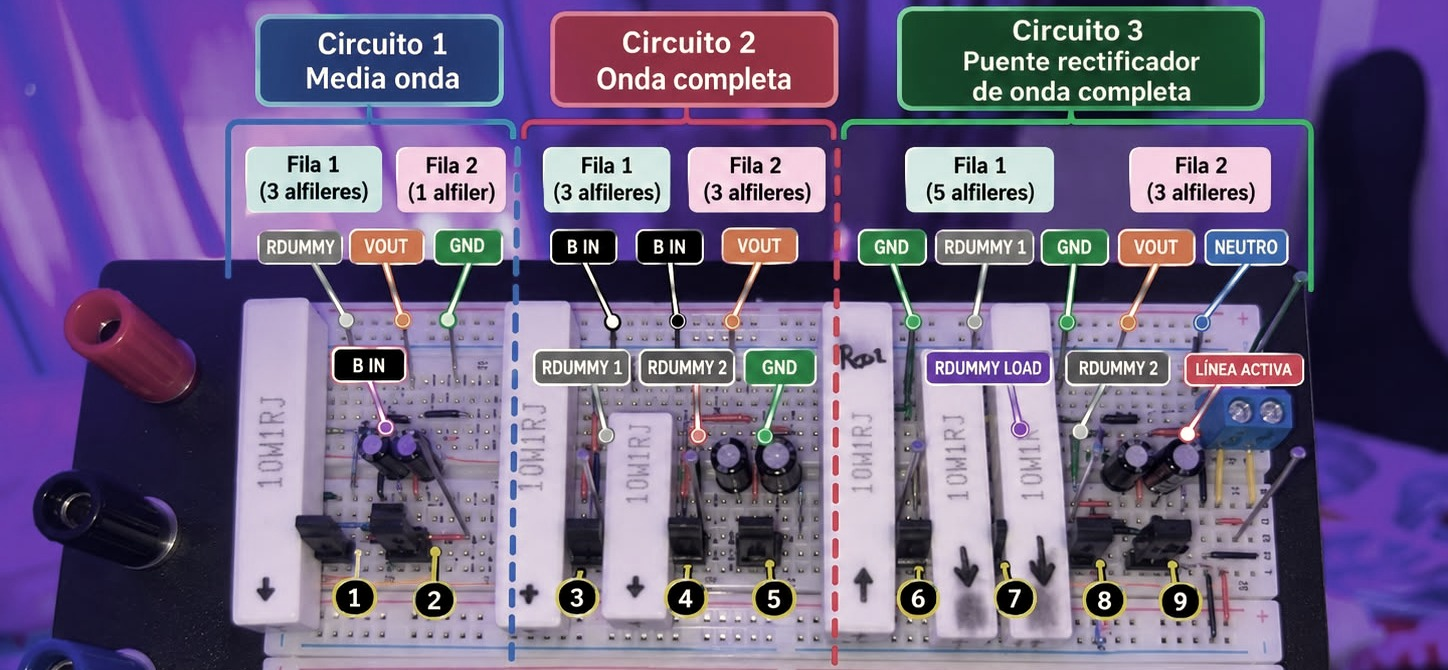
\includegraphics[width=0.9\textwidth]{img/montaje.jpg}
  \caption{Montaje físico de los tres rectificadores con los switches SW$_1$ a SW$_9$ y los puntos de medición.}
  \label{fig:montaje}
\end{figure*}

% ---- Bloques modulares -------------------------------------------------
\begin{figure*}[!t]
  \centering
  \subfloat[Switch en paralelo con $R_{D}$.\label{fig:bloque_dummy}]{%
    \resizebox{0.46\textwidth}{!}{\input{sub_files/circuitos/c4-bloque-dummy}}}
  \hfill
  \subfloat[Switch selector de capacitor en paralelo con $R_L$.\label{fig:bloque_carga}]{%
    \resizebox{0.50\textwidth}{!}{\input{sub_files/circuitos/c5-bloque-carga}}}
  \caption{Bloques modulares de los switches y su convención de estados.}
  \label{fig:bloques}
\end{figure*}

% ---- Circuitos adaptados ----------------------------------------------
\begin{figure*}[!t]
  \centering
  \subfloat[Media onda (SW$_1$, SW$_2$).\label{fig:adapt_media}]{%
    \resizebox{0.32\textwidth}{!}{\input{sub_files/circuitos/c6-media-onda-adaptado}}}
  \hfill
  \subfloat[Onda completa con tab central (SW$_3$, SW$_4$, SW$_5$).\label{fig:adapt_tab}]{%
    \resizebox{0.62\textwidth}{!}{\input{sub_files/circuitos/c7-tab-central-adaptado}}}
  \\[2ex]
  \subfloat[Puente rectificador (SW$_6$ a SW$_9$).\label{fig:adapt_puente}]{%
    \resizebox{0.62\textwidth}{!}{\input{sub_files/circuitos/c8-puente-adaptado}}}
  \caption{Circuitos adaptados con resistencias dummy y selector de capacitores.}
  \label{fig:adaptados}
\end{figure*}

% ---- Tablas de mediciones (C cerrado, A abierto, I izquierda, D derecha) --
\begin{table}[!t]
  \centering
  \footnotesize
  \caption{Mediciones del rectificador de media onda (C: cerrado, A: abierto, I: izquierda, D: derecha).}
  \label{tab:med_media}
  \begin{tabular}{llccl}
    \toprule
    \textbf{Carga} & \textbf{Medición} & \textbf{SW$_1$} & \textbf{SW$_2$} & \textbf{Archivo} \\ \midrule
    \multirow{2}{*}{$R_L$}               & $R_L$    & C & A & 1110.csv \\
                                         & $R_{D1}$ & A & A & 1120.csv \\ \midrule
    \multirow{2}{*}{$R_L \parallel C_1$} & $R_L$    & C & I & 1210.csv \\
                                         & $R_{D1}$ & A & I & 1220.csv \\ \midrule
    \multirow{2}{*}{$R_L \parallel C_2$} & $R_L$    & C & D & 1310.csv \\
                                         & $R_{D1}$ & A & D & 1320.csv \\ \bottomrule
  \end{tabular}
\end{table}

\begin{table}[!t]
  \centering
  \footnotesize
  \caption{Mediciones del rectificador de onda completa con tab central (C: cerrado, A: abierto, I: izquierda, D: derecha).}
  \label{tab:med_tab}
  \begin{tabular}{llcccl}
    \toprule
    \textbf{Carga} & \textbf{Medición} & \textbf{SW$_3$} & \textbf{SW$_4$} & \textbf{SW$_5$} & \textbf{Archivo} \\ \midrule
    \multirow{3}{*}{$R_L$}               & $R_L$    & C & C & A & 2110.csv \\
                                         & $R_{D3}$ & A & A & A & 2120.csv \\
                                         & $R_{D4}$ & A & A & A & 2130.csv \\ \midrule
    \multirow{3}{*}{$R_L \parallel C_1$} & $R_L$    & C & C & I & 2210.csv \\
                                         & $R_{D3}$ & A & A & I & 2220.csv \\
                                         & $R_{D4}$ & A & A & I & 2230.csv \\ \midrule
    \multirow{3}{*}{$R_L \parallel C_2$} & $R_L$    & C & C & D & 2310.csv \\
                                         & $R_{D3}$ & A & A & D & 2320.csv \\
                                         & $R_{D4}$ & A & A & D & 2330.csv \\ \bottomrule
  \end{tabular}
\end{table}

\begin{table}[!t]
  \centering
  \footnotesize
  \caption{Mediciones del puente rectificador (C: cerrado, A: abierto, I: izquierda, D: derecha).}
  \label{tab:med_puente}
  \begin{tabular}{llccccl}
    \toprule
    \textbf{Carga} & \textbf{Medición} & \textbf{SW$_6$} & \textbf{SW$_7$} & \textbf{SW$_8$} & \textbf{SW$_9$} & \textbf{Archivo} \\ \midrule
    \multirow{4}{*}{$R_L$}               & $R_L$    & C & C & C & A & 3110.csv \\
                                         & $R_{D6}$ & A & A & C & A & 3120.csv \\
                                         & $R_{D7}$ & A & A & C & A & 3130.csv \\
                                         & $R_{D8}$ & C & C & A & A & 3140.csv \\ \midrule
    \multirow{4}{*}{$R_L \parallel C_1$} & $R_L$    & C & C & C & I & 3210.csv \\
                                         & $R_{D6}$ & A & A & C & I & 3220.csv \\
                                         & $R_{D7}$ & A & A & C & I & 3230.csv \\
                                         & $R_{D8}$ & C & C & A & I & 3240.csv \\ \midrule
    \multirow{4}{*}{$R_L \parallel C_2$} & $R_L$    & C & C & C & D & 3310.csv \\
                                         & $R_{D6}$ & A & A & C & D & 3320.csv \\
                                         & $R_{D7}$ & A & A & C & D & 3330.csv \\
                                         & $R_{D8}$ & C & C & A & D & 3340.csv \\ \bottomrule
  \end{tabular}
\end{table}

% =====================================================================
% =====================================================================
%  Macros de los circuitos (CircuiTikZ ya se carga en el main con [american]).
%  Se puede \input en cualquier parte del documento antes de los circuitos.
% =====================================================================
\ctikzset{voltage dir=RP}

% ---- Etiquetas editables (cambiar con \renewcommand dentro de cada figura) ----
\providecommand{\etqFuente}{v_s}            % senal de entrada
\providecommand{\etqSec}{v_p}               % cada mitad del secundario (tab central)
\providecommand{\etqCarga}{R_L}             % resistencia de carga (reostato)
\providecommand{\etqSalida}{V_{out}}        % voltaje de salida
\providecommand{\etqCuno}{C_1}
\providecommand{\etqCdos}{C_2}
\providecommand{\etqRdummy}{1\,\Omega}      % valor de la R dummy
\providecommand{\sepCarga}{3.2}             % distancia R_L -> selector de C (subir si las etiquetas son largas)

% ---- Bloque: switch en paralelo con R dummy ----------------------------
% \dummyH{punto inicial}{largo}{switch}{resistencia}  horizontal, hacia la derecha
% \dummyV{punto inicial}{largo}{switch}{resistencia}  vertical, hacia abajo
\providecommand{\dummyH}[4]{%
  \draw (#1) to[short,*-] ++(0,0.6) to[nos, l={$#3$}] ++(#2,0) -- ++(0,-1.2)
             to[R, l={$#4$}] ++(-#2,0) -- ++(0,0.6);
  \draw (#1) ++(#2,0) node[circ]{};
}
\providecommand{\dummyV}[4]{%
  \draw (#1) to[short,*-] ++(-0.6,0) to[nos, l_={$#3$}] ++(0,-#2) -- ++(1.2,0)
             to[R, l_={$#4$}] ++(0,#2) -- ++(-0.6,0);
  \draw (#1) ++(0,-#2) node[circ]{};
}

% ---- Bloque: carga R_L con selector de capacitor en paralelo -----------
% \carga{nodo superior}{altura}{switch}
%   brazo al centro = abierto, izquierda = C1, derecha = C2
%   deja definida la coordenada (B) = nodo inferior de R_L
%   (flechas escritas como stealth-stealth para no chocar con babel-spanish)
\providecommand{\carga}[3]{%
  \coordinate (T) at (#1);
  \draw (T) to[vR, l_={$\etqCarga$}, v^={$\etqSalida$}, *-*] ++(0,-#2) coordinate(B);
  \draw (T) -- ++(\sepCarga,0) node[circ]{} coordinate(P) node[above]{$#3$};
  \draw[line width=0.8pt] (P) -- ++(0,-0.75);                          % brazo (abierto)
  \draw[stealth-stealth, thin] (P) ++(-125:0.55) arc[start angle=-125, end angle=-55, radius=0.55];
  \draw (P) ++(-0.7,-0.9) coordinate(K1) to[C, l_={$\etqCuno$}, o-*] (K1 |- B);
  \draw (P) ++( 0.7,-0.9) coordinate(K2) to[C, l={$\etqCdos$}, o-] (K2 |- B);
  \draw (B) -- (K2 |- B);
}

% ---- Transformador con tab central -------------------------------------
\providecommand{\trafoTab}{%
  \draw (0,0) to[sV, l={$\etqFuente$}] (0,4) -- (1.5,4) to[cute inductor] (1.5,0) -- (0,0);
  \draw[line width=1pt] (1.95,0.6) -- (1.95,3.4) (2.15,0.6) -- (2.15,3.4);
  \draw (2.6,4) to[cute inductor, mirror, l={$\etqSec$}] (2.6,2)
                to[cute inductor, mirror, l={$\etqSec$}] (2.6,0);
}


% ---- Montaje fisico ---------------------------------------------------
\begin{figure*}[!t]
  \centering
  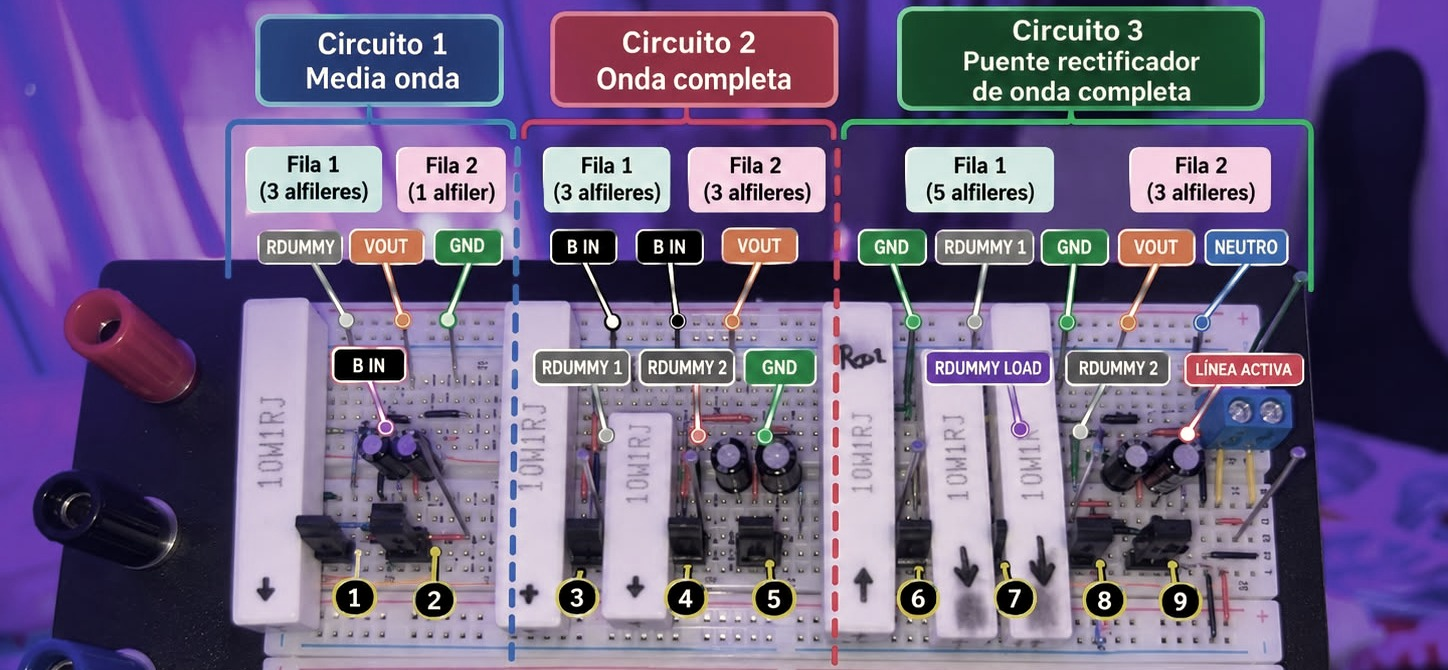
\includegraphics[width=0.9\textwidth]{img/montaje.jpg}
  \caption{Montaje físico de los tres rectificadores con los switches SW$_1$ a SW$_9$ y los puntos de medición.}
  \label{fig:montaje}
\end{figure*}

% ---- Bloques modulares -------------------------------------------------
\begin{figure*}[!t]
  \centering
  \subfloat[Switch en paralelo con $R_{D}$.\label{fig:bloque_dummy}]{%
    \resizebox{0.46\textwidth}{!}{% 4) Bloque: R dummy en paralelo con un switch
\begin{circuitikz}
  \draw (0,0) to[short,o-] (1,0);
  \dummyH{1,0}{2.4}{SW}{R_D = \etqRdummy}
  \draw (3.4,0) to[short,-o] (4.4,0);
  \node[right] at (5,0) {%
    \begin{tabular}{ll}
      \hline
      \textbf{SW} & \textbf{Resistencia vista} \\ \hline
      Cerrado & $0\,\Omega$ ($R_D$ en corto) \\
      Abierto & $R_D = \etqRdummy$ \\ \hline
    \end{tabular}};
\end{circuitikz}
}}
  \hfill
  \subfloat[Switch selector de capacitor en paralelo con $R_L$.\label{fig:bloque_carga}]{%
    \resizebox{0.50\textwidth}{!}{% 5) Bloque: carga R_L con switch selector de capacitor en paralelo
\begin{circuitikz}
  \draw (-1,2.8) to[short,o-] (0,2.8);
  \carga{0,2.8}{2.8}{SW}
  \draw (-1,0) to[short,o-] (B);
  \node[right] at (5.4,1.4) {%
    \begin{tabular}{ll}
      \hline
      \textbf{SW} & \textbf{Carga vista} \\ \hline
      Abierto   & $\etqCarga$ \\
      Izquierda & $\etqCarga \parallel \etqCuno$ \\
      Derecha   & $\etqCarga \parallel \etqCdos$ \\ \hline
    \end{tabular}};
\end{circuitikz}
}}
  \caption{Bloques modulares de los switches y su convención de estados.}
  \label{fig:bloques}
\end{figure*}

% ---- Circuitos adaptados ----------------------------------------------
\begin{figure*}[!t]
  \centering
  \subfloat[Media onda (SW$_1$, SW$_2$).\label{fig:adapt_media}]{%
    \resizebox{0.32\textwidth}{!}{% 6) Media onda adaptado: SW_1 (dummy entre R_L y tierra), SW_2 (selector de C)
\begin{circuitikz}
  \draw (0,0) to[sV, l={$\etqFuente$}] (0,5) to[D*, l=$D_1$] (3,5);
  \carga{3,5}{2.8}{SW_2}
  \dummyV{3,2.2}{2.2}{SW_1}{R_{D1}}
  \draw (0,0) -- (3,0);
  \draw (1.5,0) node[ground]{};
\end{circuitikz}
}}
  \hfill
  \subfloat[Onda completa con tab central (SW$_3$, SW$_4$, SW$_5$).\label{fig:adapt_tab}]{%
    \resizebox{0.62\textwidth}{!}{% 7) Tab central adaptado: SW_3 y SW_4 (dummies de cada rama), SW_5 (selector de C)
\begin{circuitikz}
  \trafoTab
  \draw (2.6,4) to[D*, l=$D_1$] (4.4,4) -- (4.8,4);
  \dummyH{4.8,4}{2.2}{SW_3}{R_{D3}}
  \draw (7,4) -- (8,4) -- (8,0);
  \draw (2.6,0) to[D*, l_=$D_2$] (4.4,0) -- (4.8,0);
  \dummyH{4.8,0}{2.2}{SW_4}{R_{D4}}
  \draw (7,0) -- (8,0);
  \draw (2.6,2) to[short,*-] (3.4,2) node[ground]{};
  \draw (8,2) to[short,*-] (9.6,2);
  \carga{9.6,2}{3.5}{SW_5}
  \draw (B) node[ground]{};
\end{circuitikz}
}}
  \\[2ex]
  \subfloat[Puente rectificador (SW$_6$ a SW$_9$).\label{fig:adapt_puente}]{%
    \resizebox{0.62\textwidth}{!}{% 8) Puente adaptado: dummies a tierra. SW_6 y SW_7 (ramas de diodos),
%    SW_8 (en serie con la carga), SW_9 (selector de C)
\begin{circuitikz}
  % ramas de diodos: la corriente sube desde tierra por la dummy y entra al anodo
  \dummyV{0,2.2}{2.2}{SW_6}{R_{D6}}
  \draw (0,2.2) to[D*, l=$D_2$] (0,4.4) to[D*, l=$D_1$] (0,6.6);
  \dummyV{4,2.2}{2.2}{SW_7}{R_{D7}}
  \draw (4,2.2) to[D*, l=$D_4$] (4,4.4) to[D*, l=$D_3$] (4,6.6);
  \draw (0,4.4) to[sV, l={$\etqFuente$}, *-*] (4,4.4);
  % carga y su dummy
  \draw (0,6.6) to[short,-*] (4,6.6) -- (8,6.6);
  \carga{8,6.6}{4.4}{SW_9}
  \dummyV{8,2.2}{2.2}{SW_8}{R_{D8}}
  % tierra
  \draw (0,0) -- (8,0);
  \draw (2,0) node[ground]{};
\end{circuitikz}
}}
  \caption{Circuitos adaptados con resistencias dummy y selector de capacitores.}
  \label{fig:adaptados}
\end{figure*}

% ---- Tablas de mediciones (C cerrado, A abierto, I izquierda, D derecha) --
\begin{table}[!t]
  \centering
  \footnotesize
  \caption{Mediciones del rectificador de media onda (C: cerrado, A: abierto, I: izquierda, D: derecha).}
  \label{tab:med_media}
  \begin{tabular}{llccl}
    \toprule
    \textbf{Carga} & \textbf{Medición} & \textbf{SW$_1$} & \textbf{SW$_2$} & \textbf{Archivo} \\ \midrule
    \multirow{2}{*}{$R_L$}               & $R_L$    & C & A & 1110.csv \\
                                         & $R_{D1}$ & A & A & 1120.csv \\ \midrule
    \multirow{2}{*}{$R_L \parallel C_1$} & $R_L$    & C & I & 1210.csv \\
                                         & $R_{D1}$ & A & I & 1220.csv \\ \midrule
    \multirow{2}{*}{$R_L \parallel C_2$} & $R_L$    & C & D & 1310.csv \\
                                         & $R_{D1}$ & A & D & 1320.csv \\ \bottomrule
  \end{tabular}
\end{table}

\begin{table}[!t]
  \centering
  \footnotesize
  \caption{Mediciones del rectificador de onda completa con tab central (C: cerrado, A: abierto, I: izquierda, D: derecha).}
  \label{tab:med_tab}
  \begin{tabular}{llcccl}
    \toprule
    \textbf{Carga} & \textbf{Medición} & \textbf{SW$_3$} & \textbf{SW$_4$} & \textbf{SW$_5$} & \textbf{Archivo} \\ \midrule
    \multirow{3}{*}{$R_L$}               & $R_L$    & C & C & A & 2110.csv \\
                                         & $R_{D3}$ & A & A & A & 2120.csv \\
                                         & $R_{D4}$ & A & A & A & 2130.csv \\ \midrule
    \multirow{3}{*}{$R_L \parallel C_1$} & $R_L$    & C & C & I & 2210.csv \\
                                         & $R_{D3}$ & A & A & I & 2220.csv \\
                                         & $R_{D4}$ & A & A & I & 2230.csv \\ \midrule
    \multirow{3}{*}{$R_L \parallel C_2$} & $R_L$    & C & C & D & 2310.csv \\
                                         & $R_{D3}$ & A & A & D & 2320.csv \\
                                         & $R_{D4}$ & A & A & D & 2330.csv \\ \bottomrule
  \end{tabular}
\end{table}

\begin{table}[!t]
  \centering
  \footnotesize
  \caption{Mediciones del puente rectificador (C: cerrado, A: abierto, I: izquierda, D: derecha).}
  \label{tab:med_puente}
  \begin{tabular}{llccccl}
    \toprule
    \textbf{Carga} & \textbf{Medición} & \textbf{SW$_6$} & \textbf{SW$_7$} & \textbf{SW$_8$} & \textbf{SW$_9$} & \textbf{Archivo} \\ \midrule
    \multirow{4}{*}{$R_L$}               & $R_L$    & C & C & C & A & 3110.csv \\
                                         & $R_{D6}$ & A & A & C & A & 3120.csv \\
                                         & $R_{D7}$ & A & A & C & A & 3130.csv \\
                                         & $R_{D8}$ & C & C & A & A & 3140.csv \\ \midrule
    \multirow{4}{*}{$R_L \parallel C_1$} & $R_L$    & C & C & C & I & 3210.csv \\
                                         & $R_{D6}$ & A & A & C & I & 3220.csv \\
                                         & $R_{D7}$ & A & A & C & I & 3230.csv \\
                                         & $R_{D8}$ & C & C & A & I & 3240.csv \\ \midrule
    \multirow{4}{*}{$R_L \parallel C_2$} & $R_L$    & C & C & C & D & 3310.csv \\
                                         & $R_{D6}$ & A & A & C & D & 3320.csv \\
                                         & $R_{D7}$ & A & A & C & D & 3330.csv \\
                                         & $R_{D8}$ & C & C & A & D & 3340.csv \\ \bottomrule
  \end{tabular}
\end{table}

% =====================================================================
% =====================================================================
%  Macros de los circuitos (CircuiTikZ ya se carga en el main con [american]).
%  Se puede \input en cualquier parte del documento antes de los circuitos.
% =====================================================================
\ctikzset{voltage dir=RP}

% ---- Etiquetas editables (cambiar con \renewcommand dentro de cada figura) ----
\providecommand{\etqFuente}{v_s}            % senal de entrada
\providecommand{\etqSec}{v_p}               % cada mitad del secundario (tab central)
\providecommand{\etqCarga}{R_L}             % resistencia de carga (reostato)
\providecommand{\etqSalida}{V_{out}}        % voltaje de salida
\providecommand{\etqCuno}{C_1}
\providecommand{\etqCdos}{C_2}
\providecommand{\etqRdummy}{1\,\Omega}      % valor de la R dummy
\providecommand{\sepCarga}{3.2}             % distancia R_L -> selector de C (subir si las etiquetas son largas)

% ---- Bloque: switch en paralelo con R dummy ----------------------------
% \dummyH{punto inicial}{largo}{switch}{resistencia}  horizontal, hacia la derecha
% \dummyV{punto inicial}{largo}{switch}{resistencia}  vertical, hacia abajo
\providecommand{\dummyH}[4]{%
  \draw (#1) to[short,*-] ++(0,0.6) to[nos, l={$#3$}] ++(#2,0) -- ++(0,-1.2)
             to[R, l={$#4$}] ++(-#2,0) -- ++(0,0.6);
  \draw (#1) ++(#2,0) node[circ]{};
}
\providecommand{\dummyV}[4]{%
  \draw (#1) to[short,*-] ++(-0.6,0) to[nos, l_={$#3$}] ++(0,-#2) -- ++(1.2,0)
             to[R, l_={$#4$}] ++(0,#2) -- ++(-0.6,0);
  \draw (#1) ++(0,-#2) node[circ]{};
}

% ---- Bloque: carga R_L con selector de capacitor en paralelo -----------
% \carga{nodo superior}{altura}{switch}
%   brazo al centro = abierto, izquierda = C1, derecha = C2
%   deja definida la coordenada (B) = nodo inferior de R_L
%   (flechas escritas como stealth-stealth para no chocar con babel-spanish)
\providecommand{\carga}[3]{%
  \coordinate (T) at (#1);
  \draw (T) to[vR, l_={$\etqCarga$}, v^={$\etqSalida$}, *-*] ++(0,-#2) coordinate(B);
  \draw (T) -- ++(\sepCarga,0) node[circ]{} coordinate(P) node[above]{$#3$};
  \draw[line width=0.8pt] (P) -- ++(0,-0.75);                          % brazo (abierto)
  \draw[stealth-stealth, thin] (P) ++(-125:0.55) arc[start angle=-125, end angle=-55, radius=0.55];
  \draw (P) ++(-0.7,-0.9) coordinate(K1) to[C, l_={$\etqCuno$}, o-*] (K1 |- B);
  \draw (P) ++( 0.7,-0.9) coordinate(K2) to[C, l={$\etqCdos$}, o-] (K2 |- B);
  \draw (B) -- (K2 |- B);
}

% ---- Transformador con tab central -------------------------------------
\providecommand{\trafoTab}{%
  \draw (0,0) to[sV, l={$\etqFuente$}] (0,4) -- (1.5,4) to[cute inductor] (1.5,0) -- (0,0);
  \draw[line width=1pt] (1.95,0.6) -- (1.95,3.4) (2.15,0.6) -- (2.15,3.4);
  \draw (2.6,4) to[cute inductor, mirror, l={$\etqSec$}] (2.6,2)
                to[cute inductor, mirror, l={$\etqSec$}] (2.6,0);
}


% ---- Montaje fisico ---------------------------------------------------
\begin{figure*}[!t]
  \centering
  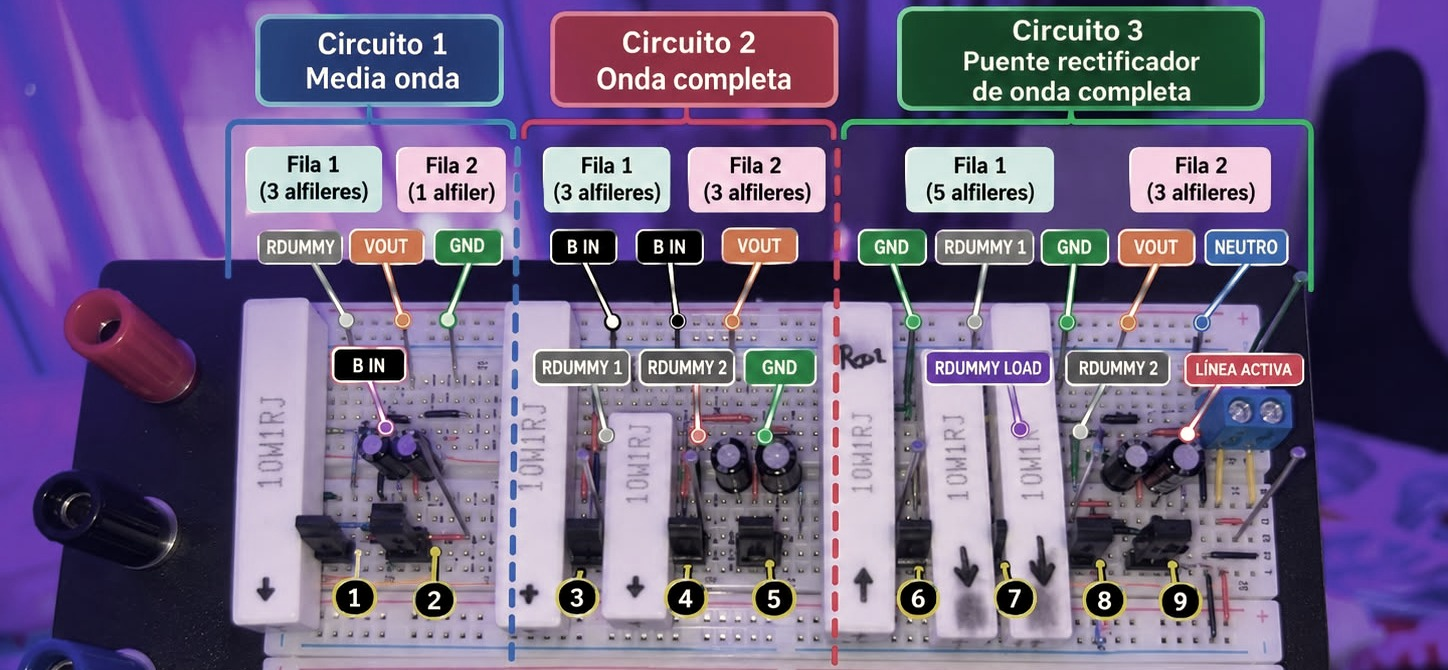
\includegraphics[width=0.9\textwidth]{img/montaje.jpg}
  \caption{Montaje físico de los tres rectificadores con los switches SW$_1$ a SW$_9$ y los puntos de medición.}
  \label{fig:montaje}
\end{figure*}

% ---- Bloques modulares -------------------------------------------------
\begin{figure*}[!t]
  \centering
  \subfloat[Switch en paralelo con $R_{D}$.\label{fig:bloque_dummy}]{%
    \resizebox{0.46\textwidth}{!}{% 4) Bloque: R dummy en paralelo con un switch
\begin{circuitikz}
  \draw (0,0) to[short,o-] (1,0);
  \dummyH{1,0}{2.4}{SW}{R_D = \etqRdummy}
  \draw (3.4,0) to[short,-o] (4.4,0);
  \node[right] at (5,0) {%
    \begin{tabular}{ll}
      \hline
      \textbf{SW} & \textbf{Resistencia vista} \\ \hline
      Cerrado & $0\,\Omega$ ($R_D$ en corto) \\
      Abierto & $R_D = \etqRdummy$ \\ \hline
    \end{tabular}};
\end{circuitikz}
}}
  \hfill
  \subfloat[Switch selector de capacitor en paralelo con $R_L$.\label{fig:bloque_carga}]{%
    \resizebox{0.50\textwidth}{!}{% 5) Bloque: carga R_L con switch selector de capacitor en paralelo
\begin{circuitikz}
  \draw (-1,2.8) to[short,o-] (0,2.8);
  \carga{0,2.8}{2.8}{SW}
  \draw (-1,0) to[short,o-] (B);
  \node[right] at (5.4,1.4) {%
    \begin{tabular}{ll}
      \hline
      \textbf{SW} & \textbf{Carga vista} \\ \hline
      Abierto   & $\etqCarga$ \\
      Izquierda & $\etqCarga \parallel \etqCuno$ \\
      Derecha   & $\etqCarga \parallel \etqCdos$ \\ \hline
    \end{tabular}};
\end{circuitikz}
}}
  \caption{Bloques modulares de los switches y su convención de estados.}
  \label{fig:bloques}
\end{figure*}

% ---- Circuitos adaptados ----------------------------------------------
\begin{figure*}[!t]
  \centering
  \subfloat[Media onda (SW$_1$, SW$_2$).\label{fig:adapt_media}]{%
    \resizebox{0.32\textwidth}{!}{% 6) Media onda adaptado: SW_1 (dummy entre R_L y tierra), SW_2 (selector de C)
\begin{circuitikz}
  \draw (0,0) to[sV, l={$\etqFuente$}] (0,5) to[D*, l=$D_1$] (3,5);
  \carga{3,5}{2.8}{SW_2}
  \dummyV{3,2.2}{2.2}{SW_1}{R_{D1}}
  \draw (0,0) -- (3,0);
  \draw (1.5,0) node[ground]{};
\end{circuitikz}
}}
  \hfill
  \subfloat[Onda completa con tab central (SW$_3$, SW$_4$, SW$_5$).\label{fig:adapt_tab}]{%
    \resizebox{0.62\textwidth}{!}{% 7) Tab central adaptado: SW_3 y SW_4 (dummies de cada rama), SW_5 (selector de C)
\begin{circuitikz}
  \trafoTab
  \draw (2.6,4) to[D*, l=$D_1$] (4.4,4) -- (4.8,4);
  \dummyH{4.8,4}{2.2}{SW_3}{R_{D3}}
  \draw (7,4) -- (8,4) -- (8,0);
  \draw (2.6,0) to[D*, l_=$D_2$] (4.4,0) -- (4.8,0);
  \dummyH{4.8,0}{2.2}{SW_4}{R_{D4}}
  \draw (7,0) -- (8,0);
  \draw (2.6,2) to[short,*-] (3.4,2) node[ground]{};
  \draw (8,2) to[short,*-] (9.6,2);
  \carga{9.6,2}{3.5}{SW_5}
  \draw (B) node[ground]{};
\end{circuitikz}
}}
  \\[2ex]
  \subfloat[Puente rectificador (SW$_6$ a SW$_9$).\label{fig:adapt_puente}]{%
    \resizebox{0.62\textwidth}{!}{% 8) Puente adaptado: dummies a tierra. SW_6 y SW_7 (ramas de diodos),
%    SW_8 (en serie con la carga), SW_9 (selector de C)
\begin{circuitikz}
  % ramas de diodos: la corriente sube desde tierra por la dummy y entra al anodo
  \dummyV{0,2.2}{2.2}{SW_6}{R_{D6}}
  \draw (0,2.2) to[D*, l=$D_2$] (0,4.4) to[D*, l=$D_1$] (0,6.6);
  \dummyV{4,2.2}{2.2}{SW_7}{R_{D7}}
  \draw (4,2.2) to[D*, l=$D_4$] (4,4.4) to[D*, l=$D_3$] (4,6.6);
  \draw (0,4.4) to[sV, l={$\etqFuente$}, *-*] (4,4.4);
  % carga y su dummy
  \draw (0,6.6) to[short,-*] (4,6.6) -- (8,6.6);
  \carga{8,6.6}{4.4}{SW_9}
  \dummyV{8,2.2}{2.2}{SW_8}{R_{D8}}
  % tierra
  \draw (0,0) -- (8,0);
  \draw (2,0) node[ground]{};
\end{circuitikz}
}}
  \caption{Circuitos adaptados con resistencias dummy y selector de capacitores.}
  \label{fig:adaptados}
\end{figure*}

% ---- Tablas de mediciones (C cerrado, A abierto, I izquierda, D derecha) --
\begin{table}[!t]
  \centering
  \footnotesize
  \caption{Mediciones del rectificador de media onda (C: cerrado, A: abierto, I: izquierda, D: derecha).}
  \label{tab:med_media}
  \begin{tabular}{llccl}
    \toprule
    \textbf{Carga} & \textbf{Medición} & \textbf{SW$_1$} & \textbf{SW$_2$} & \textbf{Archivo} \\ \midrule
    \multirow{2}{*}{$R_L$}               & $R_L$    & C & A & 1110.csv \\
                                         & $R_{D1}$ & A & A & 1120.csv \\ \midrule
    \multirow{2}{*}{$R_L \parallel C_1$} & $R_L$    & C & I & 1210.csv \\
                                         & $R_{D1}$ & A & I & 1220.csv \\ \midrule
    \multirow{2}{*}{$R_L \parallel C_2$} & $R_L$    & C & D & 1310.csv \\
                                         & $R_{D1}$ & A & D & 1320.csv \\ \bottomrule
  \end{tabular}
\end{table}

\begin{table}[!t]
  \centering
  \footnotesize
  \caption{Mediciones del rectificador de onda completa con tab central (C: cerrado, A: abierto, I: izquierda, D: derecha).}
  \label{tab:med_tab}
  \begin{tabular}{llcccl}
    \toprule
    \textbf{Carga} & \textbf{Medición} & \textbf{SW$_3$} & \textbf{SW$_4$} & \textbf{SW$_5$} & \textbf{Archivo} \\ \midrule
    \multirow{3}{*}{$R_L$}               & $R_L$    & C & C & A & 2110.csv \\
                                         & $R_{D3}$ & A & A & A & 2120.csv \\
                                         & $R_{D4}$ & A & A & A & 2130.csv \\ \midrule
    \multirow{3}{*}{$R_L \parallel C_1$} & $R_L$    & C & C & I & 2210.csv \\
                                         & $R_{D3}$ & A & A & I & 2220.csv \\
                                         & $R_{D4}$ & A & A & I & 2230.csv \\ \midrule
    \multirow{3}{*}{$R_L \parallel C_2$} & $R_L$    & C & C & D & 2310.csv \\
                                         & $R_{D3}$ & A & A & D & 2320.csv \\
                                         & $R_{D4}$ & A & A & D & 2330.csv \\ \bottomrule
  \end{tabular}
\end{table}

\begin{table}[!t]
  \centering
  \footnotesize
  \caption{Mediciones del puente rectificador (C: cerrado, A: abierto, I: izquierda, D: derecha).}
  \label{tab:med_puente}
  \begin{tabular}{llccccl}
    \toprule
    \textbf{Carga} & \textbf{Medición} & \textbf{SW$_6$} & \textbf{SW$_7$} & \textbf{SW$_8$} & \textbf{SW$_9$} & \textbf{Archivo} \\ \midrule
    \multirow{4}{*}{$R_L$}               & $R_L$    & C & C & C & A & 3110.csv \\
                                         & $R_{D6}$ & A & A & C & A & 3120.csv \\
                                         & $R_{D7}$ & A & A & C & A & 3130.csv \\
                                         & $R_{D8}$ & C & C & A & A & 3140.csv \\ \midrule
    \multirow{4}{*}{$R_L \parallel C_1$} & $R_L$    & C & C & C & I & 3210.csv \\
                                         & $R_{D6}$ & A & A & C & I & 3220.csv \\
                                         & $R_{D7}$ & A & A & C & I & 3230.csv \\
                                         & $R_{D8}$ & C & C & A & I & 3240.csv \\ \midrule
    \multirow{4}{*}{$R_L \parallel C_2$} & $R_L$    & C & C & C & D & 3310.csv \\
                                         & $R_{D6}$ & A & A & C & D & 3320.csv \\
                                         & $R_{D7}$ & A & A & C & D & 3330.csv \\
                                         & $R_{D8}$ & C & C & A & D & 3340.csv \\ \bottomrule
  \end{tabular}
\end{table}

\end{document}
